{
\subsection{Fabrication}
In order to accurately manufacture adaptive width toolpaths using an off-the-shelf 3D printing system,
we need a model which relates the required width to process parameters such as movement speed and filament extrusion speed.
A different approach might be appropriate depending on whether the filament feeder is mounted directly on the print head (a.k.a. \emph{direct drive}) or the filament fed from the back of the printer to the print head via a \emph{Bowden tube}.
Because Bowden style 3D printing systems have the filament feeder relatively far away from the nozzle, changing the internal pressure in the system requires a large amount of filament movement, which requires a prohibitive amount of time.

\subsubsection{Back pressure compensation}
We therefore keep the internal pressure constant, and vary the movement speed instead.
%In order to accurately realize a varying bead width we vary the movement speed, while keeping the internal pressure in the system constant.
One approach would be keep the filament inflow $f$ (in \si{\milli\meter\cubed\per\second}) constant by varying movement speed accordingly \cite{Kuipers2018}.
However, that doesn't result in the intended filament outflow variation - see \cref{zero_back_pressure}.
We conjecture that the filament outflow is related to the total pressure in the system,
which depends not only on the amount of filament in between the feeder wheel and the nozzle (which we keep constant), 
but also depends on the back pressure that the previous layer exerts on the filament protruding from the nozzle.
We conjecture that the amount of back pressure is monotonically related to the requested line width and compensate for the back pressure using a simple linear model:

\begin{align}
 v(w) &= \frac{f(w)}{h w} \\ 
% f &\sim p \\
% p &= p_\text{in} + p_\text{ext} \\
% p_\text{in} &= C \\
% p_\text{ext} &\sim w \\
% p_\text{ext} &= w / w^* - 1 \\
% f &= f^* - k p_\text{ext} \\
 f(w) &= f_0 - k \left( w / w_0 - 1 \right)
 % f_0 &= v_0 w_0 h 
% v &= \frac{f^* - k p_\text{ext}}{h w} \\ 
% v &= \frac{v^* w^* h - k (w / w^* - 1)}{h w}
\end{align}
where
$v(w)$ is the movement speed as a function of requested bead width $w$,
$f(w)$ is the filament outflow,
$f_0$ is a constant reference flow,
$w_0$ is a constant reference bead width
and
$k$ is the amount of back pressure compensation.

% adapted from 5.5 Discussion on implications
% limitations of back pressure compensation
Our back pressure compensation method effectively changes the speed to realize adaptive width,
but this approach is limited, since the movement speed is constrained by acceleration considerations near bends in the toolpath~\cite{Ertay2018}.
Moreover, as the layer height is decreased the back pressure becomes larger compared to the internal pressure, which might cause the back pressure compensation method to demand prohibitively slow movement speeds.
Furthermore, the shape and filling of the previous layer might influence the amount of back pressure.
%
% direct drive & pressure advance
Accurate flow control can be further enhanced by using a direct drive hardware system and by employing \emph{pressure advance algorithms} which dynamically change the internal pressure \cite{tronvoll2019investigating}.
Conversely such a setup might benefit from some form of back pressure compensation as well.

\subsubsection{Print results}\label{print_results_section}
Using increments of $0.1$ we established that using a factor of $k=1.1$ yields satisfactory bead width variation for our setup where we use
$f_0 = v_0 w_0 h $
with
$v_0=\SI{30}{\milli\meter\per\second}$, 
$w_0=\SI{0.4}{\milli\meter}$
and
$h=\SI{0.1}{\milli\meter}$.
See \cref{back_pressure}.
The fact that the printed lines are wider than intended is compensated for using a flow reduction to \SI{90}{\percent}.
%
Test prints were performed on an unmodified Ultimaker S5 system,
with a standard  \SI{0.4}{\milli\meter} nozzle
and PLA filament.
The printing order is determined greedily by choosing the closest point of a polygonal extrusion path, or the closest of either end point in case of an open polyline extrusion path.
Because the machine instructions file format \emph{G-code} doesn't natively support adaptive width beads,
we discretize adaptive width extrusions into \SI{0.2}{\milli\meter} long segments of the average width.
The results can be viewed in \cref{prints}.


\begin{figure}
\centering
\setlength{\figwidth}{0.32\columnwidth}
\setlength{\figheight}{0.5\columnwidth}
\begin{subfigure}[t]{\figwidth}\centering
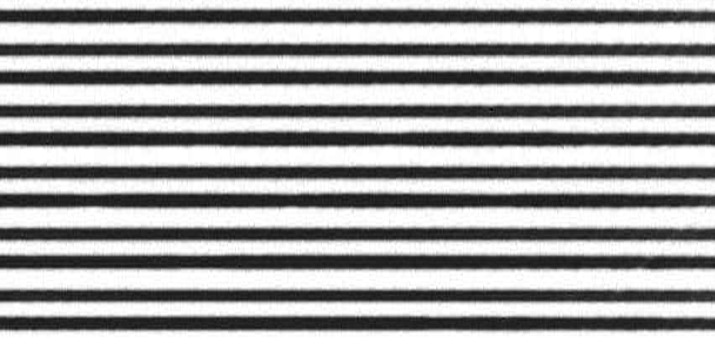
\includegraphics[angle=90,height=\figheight]{sources-validation-backpressure_0_0}
\caption{$k=0$}\label{zero_back_pressure}
\end{subfigure}
\begin{subfigure}[t]{\figwidth}\centering
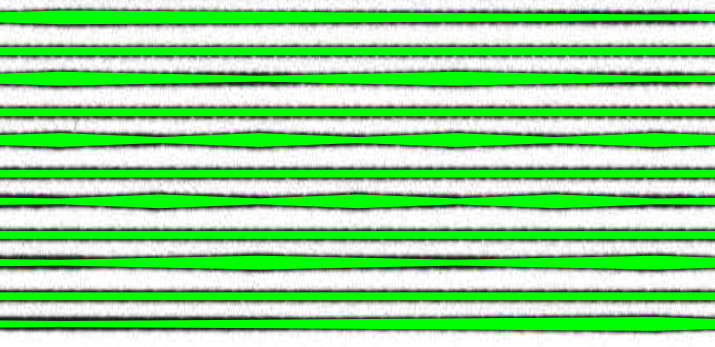
\includegraphics[angle=90,height=\figheight]{sources-validation-backpressure_1_1}
\caption{$k=1.1$}\label{back_pressure}
\end{subfigure}
\begin{subfigure}[t]{\figwidth}\centering
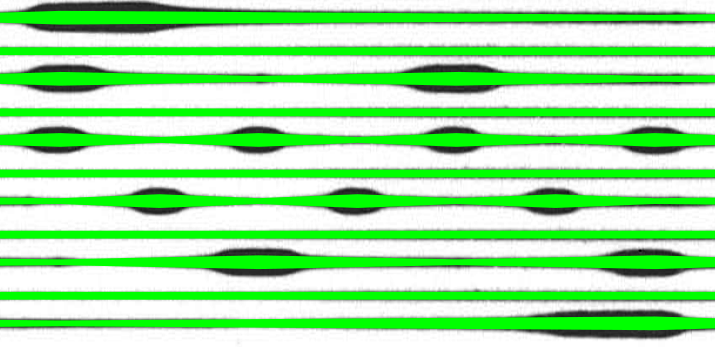
\includegraphics[angle=90,height=\figheight]{sources-validation-backpressure_2_0}
\caption{$k=2.0$}\label{too_much_back_pressure}
\end{subfigure}
\caption{
Print results (black) of the varying width test on top of a dense white raft.
Target widths in green.
\subref{zero_back_pressure} Simple flow equalization without back pressure compensation results in nearly constant bead widths.
\subref{back_pressure} A value of $k=1.1$ seems to produce good results.
}
\label{back_pressure_compensation}
\end{figure}

% discussion of print results
In \cref{print_naive} the underfill problem of the naive uniform offset approach is most prevalent for \xblackout{the Ultimaker word mark}, which negatively impacts the visual quality and the stiffness of the part.
Moreover, in the case of the spatially graded honeycomb there are several fully disconnected hexagons, which means the object falls apart when picked up.
The honeycomb print is also missing all parts which are slightly more thin than the preferred bead width $w^*$.
\Cref{print_center} still shows some underfill, but considerably less than the uniform approach.
These prints also exhibit dark regions where the translucency of the layer is less because the bead is higher.
This can be explained by inaccuracies in the back pressure compensation method, which arise for bead widths which deviate from the preferred width by a large amount.
\Cref{print_inward} diminishes the underfill nearly completely and the visual quality of these prints is more homogenous than those of the other methods.
Moreover, the absence of dark regions signifies that our proposed method is more robust against inaccuracies in the deposition system.
However, both the centered and inward distributed approach introduce transitions to a different bead count in \xblackout{the word `Delft'}, which reduces the dimensional accuracy on the outline around those locations.

\begin{figure}
\centering
\setlength{\figwidth}{\columnwidth}
\begin{subfigure}{\figwidth}\centering
\censorbox{

\includegraphics[width=\figwidth]{sources-applications-result-prints-target}
}
\caption{Outlines}\label{print_outlines}
\end{subfigure}
\begin{subfigure}{\figwidth}\centering
\censorbox{
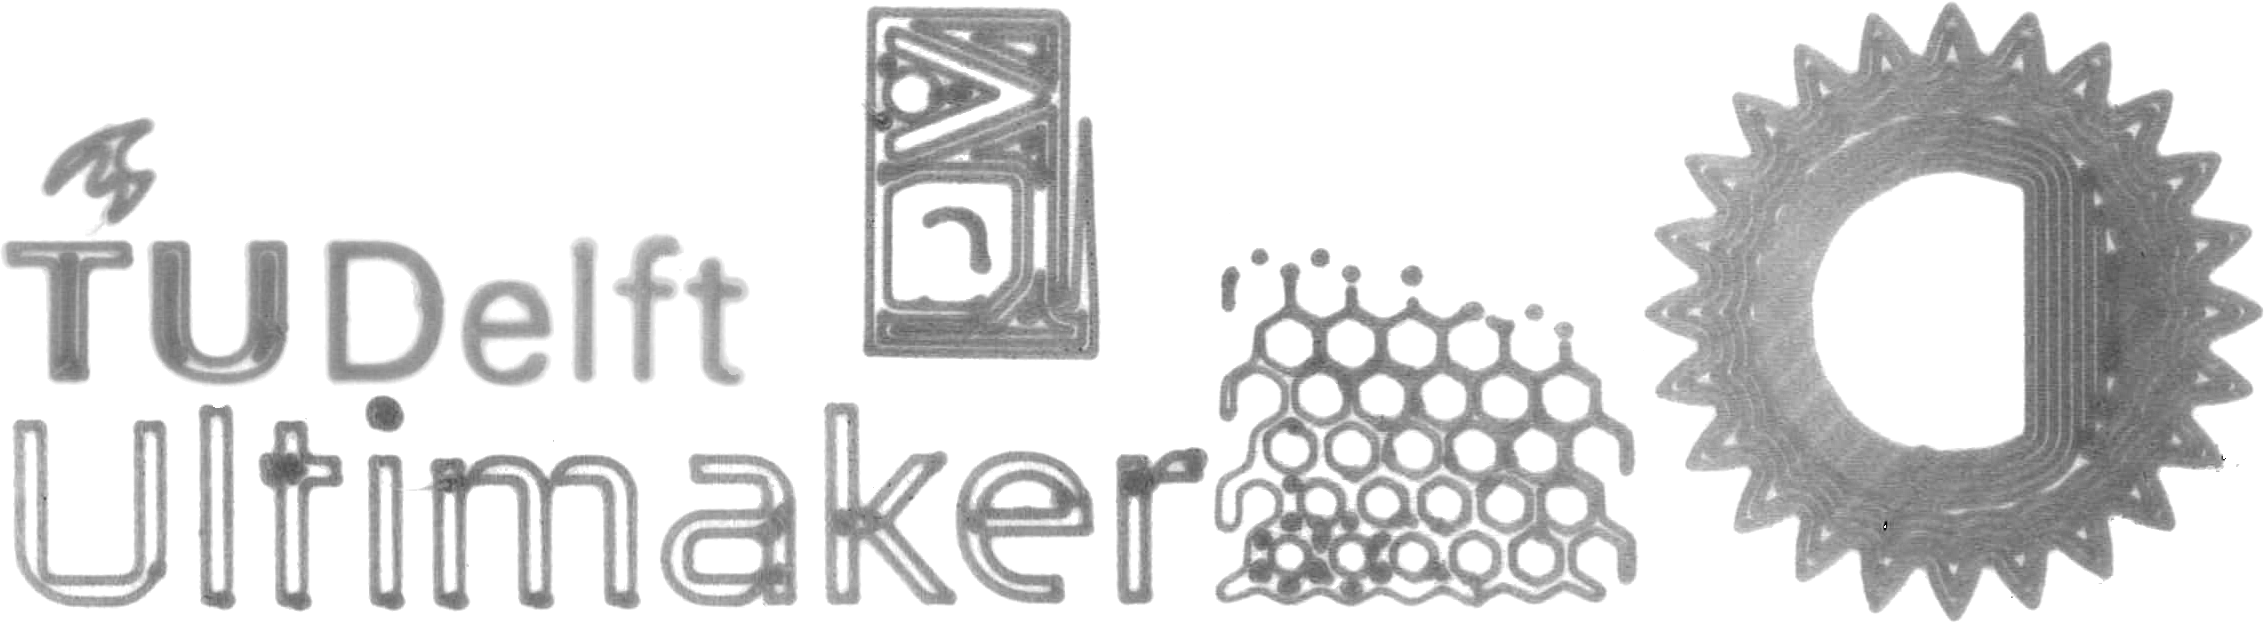
\includegraphics[width=\figwidth]{sources-applications-result-prints-naive-bw.png}
}
\caption{Uniform}\label{print_naive}
\end{subfigure}
\begin{subfigure}{\figwidth}\centering
\censorbox{
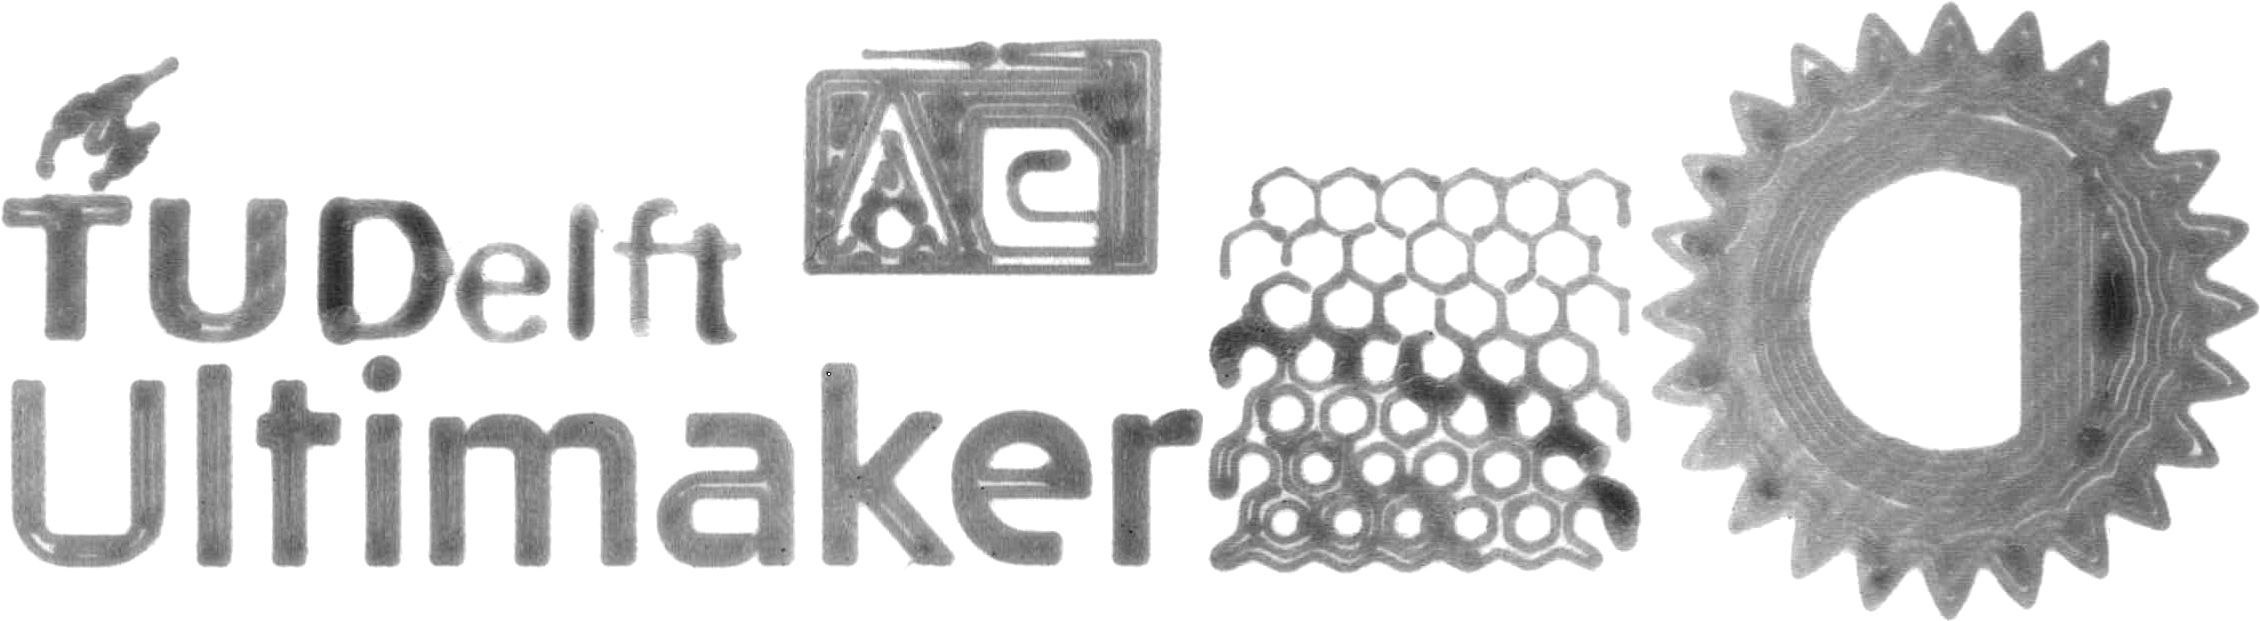
\includegraphics[width=\figwidth]{sources-applications-result-prints-center-bw.png}
}
\caption{Centered}\label{print_center}
\end{subfigure}
\begin{subfigure}{\figwidth}\centering
\censorbox{
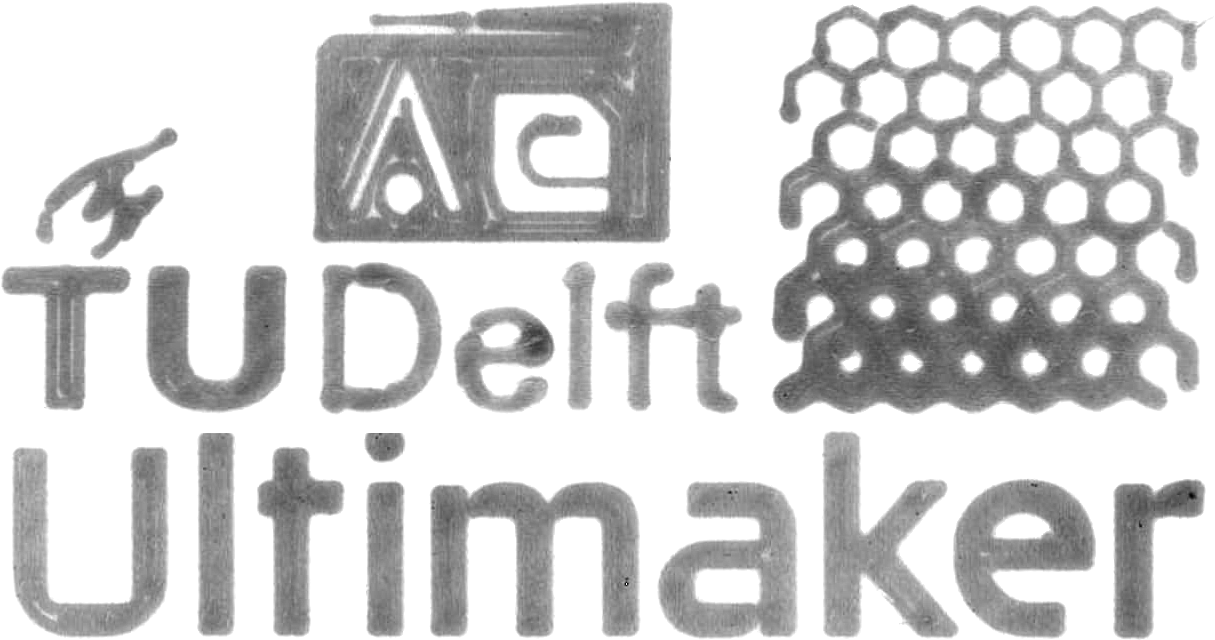
\includegraphics[width=\figwidth]{sources-applications-result-prints-inward-bw.png}
}
\caption{Inward distributed}\label{print_inward}
\end{subfigure}
\caption{
Test shapes printed using the uniform scheme, centered scheme and the inward distributed scheme.
The uniform technique produces distinct underfill areas.
The centered scheme shows some defects due to inaccurate control of extreme deposition widths.
The inward distributed scheme produces the least defects.
}
\label{prints}
\end{figure}


}
